\chapter{Phân tích thất bại và thảo luận}
\label{chap:that-bai}

Chương này hỏi: khi SemLoc (hoặc dòng LLM tự đoán) sai, nó sai thế nào và vì sao? Phân tích dùng ba lần chạy
Gemini 3.8 Flash trên tập test với nhãn đã chuẩn hóa; tín hiệu của mỗi chương trình lấy theo đa số ba lần.

\section{Sáu nhóm kết quả}
\label{sec:phan-nhom}

Mỗi chương trình được xếp vào đúng một nhóm, theo thứ tự ưu tiên: \texttt{gt\_suspect} (dòng lỗi chuẩn chưa kiểm chứng
được và mọi phương pháp trượt top-3), \texttt{guess\_right} (dòng LLM tự đoán là dòng lỗi chuẩn), \texttt{prior\_hurts}
(phổ xếp dòng lỗi hạng 1 nhưng điểm thưởng đẩy dòng đoán sai lên trên), \texttt{rescued\_by\_spectrum} (đoán sai nhưng
SemLoc vẫn có dòng lỗi trong top-3), \texttt{coverage\_only\_wins} (SemLoc trượt top-3, FailLoc+Cov trúng) và
\texttt{all\_miss}. Hình~\ref{fig:that-bai} cho số chương trình mỗi nhóm: trên \FailProgramsN{} chương trình, khoảng một
nửa được giải quyết bởi chính dòng tự đoán; bằng chứng thực thi chỉ ``cứu'' SemLoc ở \FailRescuedBySpectrumN{} chương trình.

\begin{figure}[H]
\centering
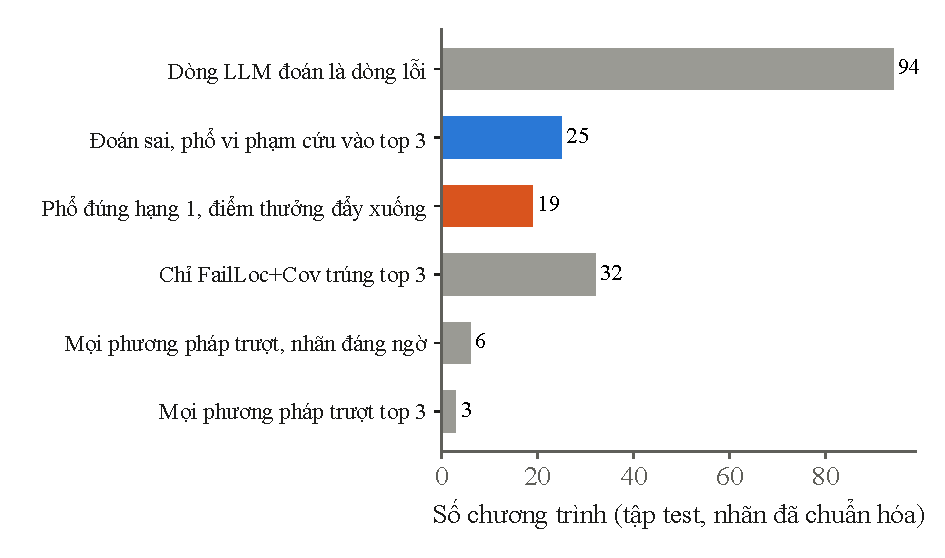
\includegraphics{../generated/vi/fig_failures.pdf}
\caption{Phân nhóm kết quả của SemLoc theo chương trình (tập test, nhãn đã chuẩn hóa, đa số ba lần chạy)}
\label{fig:that-bai}
\end{figure}

\section{Mơ hồ dòng kề cạnh và năm mẫu nguyên nhân}
\label{sec:mo-ho}

Dòng đoán lệch có hệ thống xuống dưới: trùng dòng lỗi chuẩn \OffLlmGuessZeroCount{} lần, lệch xuống một dòng
\OffLlmGuessOneCount{} lần nhưng lệch lên một dòng chỉ \OffLlmGuessMinusOneCount{} lần. Trong \FailWrongGuessN{} chương
trình đoán sai, \FailRelationHeaderBodyN{} ca có dòng đoán và dòng lỗi chuẩn là đầu một câu lệnh ghép và câu lệnh nó bảo
vệ. Chấp nhận cả hai dòng của cặp này thì Acc@1 của SemLoc tăng từ \TolSemlocAccOneExact\% lên
\TolSemlocAccOneGuardStrict\%--\TolSemlocAccOneGuardOrBody\%, của FailLoc+Cov từ \TolLlmCoverageAccOneExact\% lên
\TolLlmCoverageAccOneGuardStrict\%--\TolLlmCoverageAccOneGuardOrBody\%: quy ước gán nhãn ảnh hưởng tới Acc@1 nhiều hơn
mọi khác biệt giữa các phương pháp dùng LLM, dù thứ tự giữa chúng không đổi. Đọc mười chín ca (tối đa bốn ca mỗi nhóm,
khác khuôn mẫu) cho năm mẫu nguyên nhân:
\begin{enumerate}
\item \textbf{Dòng điều kiện và câu lệnh được bảo vệ} (phổ biến nhất): nhãn ở \texttt{if}, LLM chỉ câu lệnh bên trong
  hoặc ngược lại; đúng về ngữ nghĩa nhưng lệch một dòng.
\item \textbf{Khối lỗi nhiều dòng}: xóa dòng nào cũng sửa được; nhãn nêu một dòng, LLM chỉ dòng kia (phần lớn \texttt{prior\_hurts}).
\item \textbf{Bộ phán định chấp nhận bản sửa bù trừ}: bản sửa làm mọi kiểm thử đạt ở một dòng không có lỗi. Bản sửa trên
  dòng trống đã bị loại (\GtBlankFixDroppedN{} chương trình); vòng rà soát bác \ReviewCorrectedOverturnedN{} trong
  \GtCorrectedN{} lần bộ phán định dời nhãn.
\item \textbf{Nguyên nhân và triệu chứng trên cùng luồng dữ liệu}: nhãn ở nơi tính giá trị, LLM chỉ nơi dùng (hoặc ngược
  lại), hay lỗi là \emph{thiếu} một bước, không có ``dòng sai'' duy nhất.
\item \textbf{Dòng lỗi chuẩn đáng ngờ}: nhãn gán cho dòng khai báo hàm lồng hay cho dòng ngay trên lỗi rõ ràng.\end{enumerate}
Vì vậy không thể suy ra ``bỏ điểm thưởng thì tốt hơn'': các ca điểm thưởng ``gây hại'' gần như toàn là cặp đầu khối --
thân khối hoặc khối lỗi nhiều dòng. Điều còn thiếu là cách đánh giá chấp nhận các vị trí sửa tương đương.

\section{Thảo luận}
\label{sec:thao-luan}

\textbf{Kiểm thử đủ để gợi ý lỗi nhưng quá yếu để làm trọng tài.} Bằng chứng thực thi có ích ở top-3
(\FailRescuedBySpectrumN{} chương trình được phổ cứu, \FailCoverageOnlyWinsN{} chương trình SemLoc trượt nhưng FailLoc+Cov trúng), và
phần có ích là kiểm thử thất bại chứ không phải độ phủ (mục~\ref{sec:rq2}). Nhưng ba hiện tượng --- bước vá thử của SemLoc
không đổi thứ hạng nào, bộ phán định dời \ReviewCorrectedOverturnedN{} nhãn tới dòng bị vòng rà soát bác, và FailLoc+Verify
không cải thiện bước đề xuất --- có chung một tiêu chí: \emph{một bản sửa nhỏ tại dòng này làm mọi kiểm thử đạt}. Với
khoảng mười kiểm thử mỗi chương trình, tiêu chí này thỏa ở \PavmechReviewedOtherLineFixable\% lần thử tại các dòng ứng
viên không có lỗi (tập dev), thường bằng cách đổi một hằng số để bù cho phép tính sai ở chỗ khác, nhưng chỉ
\PavmechReviewedFaultLineFixable\% tại dòng lỗi thật (lỗi hai dòng hay lỗi thiếu mã không sửa được bằng một thay đổi nhỏ).
Đây là hiện tượng ``bản vá hợp lệ bề ngoài''~\cite{qi2015kali,smith2015cure}, nhìn từ phía định vị lỗi: bộ kiểm thử đủ
để \emph{gợi ý} lỗi ở đâu nhưng quá yếu để \emph{chứng minh} lỗi ở đâu.

\textbf{Bộ dữ liệu bão hòa.} Trên nhãn đã rà soát, FailLoc đạt Acc@3 \RqTwoReviewedAllLlmTestsAccThreeMean\%: hàm ngắn,
lỗi nhỏ, tên kiểm thử nói gần như thẳng ý định bị vi phạm; trên lỗi thật (mục~\ref{sec:rq3}) mọi phương pháp còn xa trần.
